\section{Módulo Sensor e Módulo Coordenador}
\label{Sec:5-hardware}

\subsection{XBee: configuração}
O tutorial usado para configurar a rede dos dispositivos XBee encontra-se em \cite{xbee_setup}.

As configurações utilizadas foram: 

\subsubsection{Módulo Sensor:}
\begin{itemize}
	\item Versão de Firmware:
    \begin{itemize}
    	\item Product Family: XB24-ZB
        \item Function Set: ZigBee Router AT
        \item Firmware Version: 22A7
    \end{itemize}
    \item Pad ID: BABABA
        \item Destination Address High: 13A200
        \item Destination Address Low: 40E4429B
        \item Data bits: 8
        \item Baud Rate: 9600
        \item Parity: No parity
        \item Stop Bits: One Stop Bit
\end{itemize}

\subsubsection{Módulo Coordenador:}
\begin{itemize}
	\item Versão de Firmware:
    \begin{itemize}
    	\item Product Family: XB24-ZB
        \item Function Set: ZigBee Coordinator API
        \item Firmware Version: 21A7
    \end{itemize}
    \item Pad ID: BABABA
        \item Destination Address High: 13A200
        \item Destination Address Low: 40E44285
        \item Data bits: 8
        \item Baud Rate: 9600
        \item Parity: No parity
        \item Stop Bits: One Stop Bit
\end{itemize}

\subsection{Raspberry: Sistema Operacional}

Raspberry Pi é um computador, como tal é possível usá-lo com um sistema operacional. O sistema operacional usado é o Raspian, baseado no Debian customizado para rodar no raspberry pi. Apesar de teoricamente não ser necessário o raspberry usar um sistema operacional, facilita muito o desenvolvimento tal equipamento conter uma interface amigável para seu uso.

\subsection{Raspberry: Adaptador Wifi}

Após o sistema Raspian ser instalado no cartão de memória, foi necessário configurar o adaptador Wifi (figura \ref{fig:wifi-adapter}). O modelo usado é o TP-Link TL-WN723N.

\begin{figure}[H]
\centering
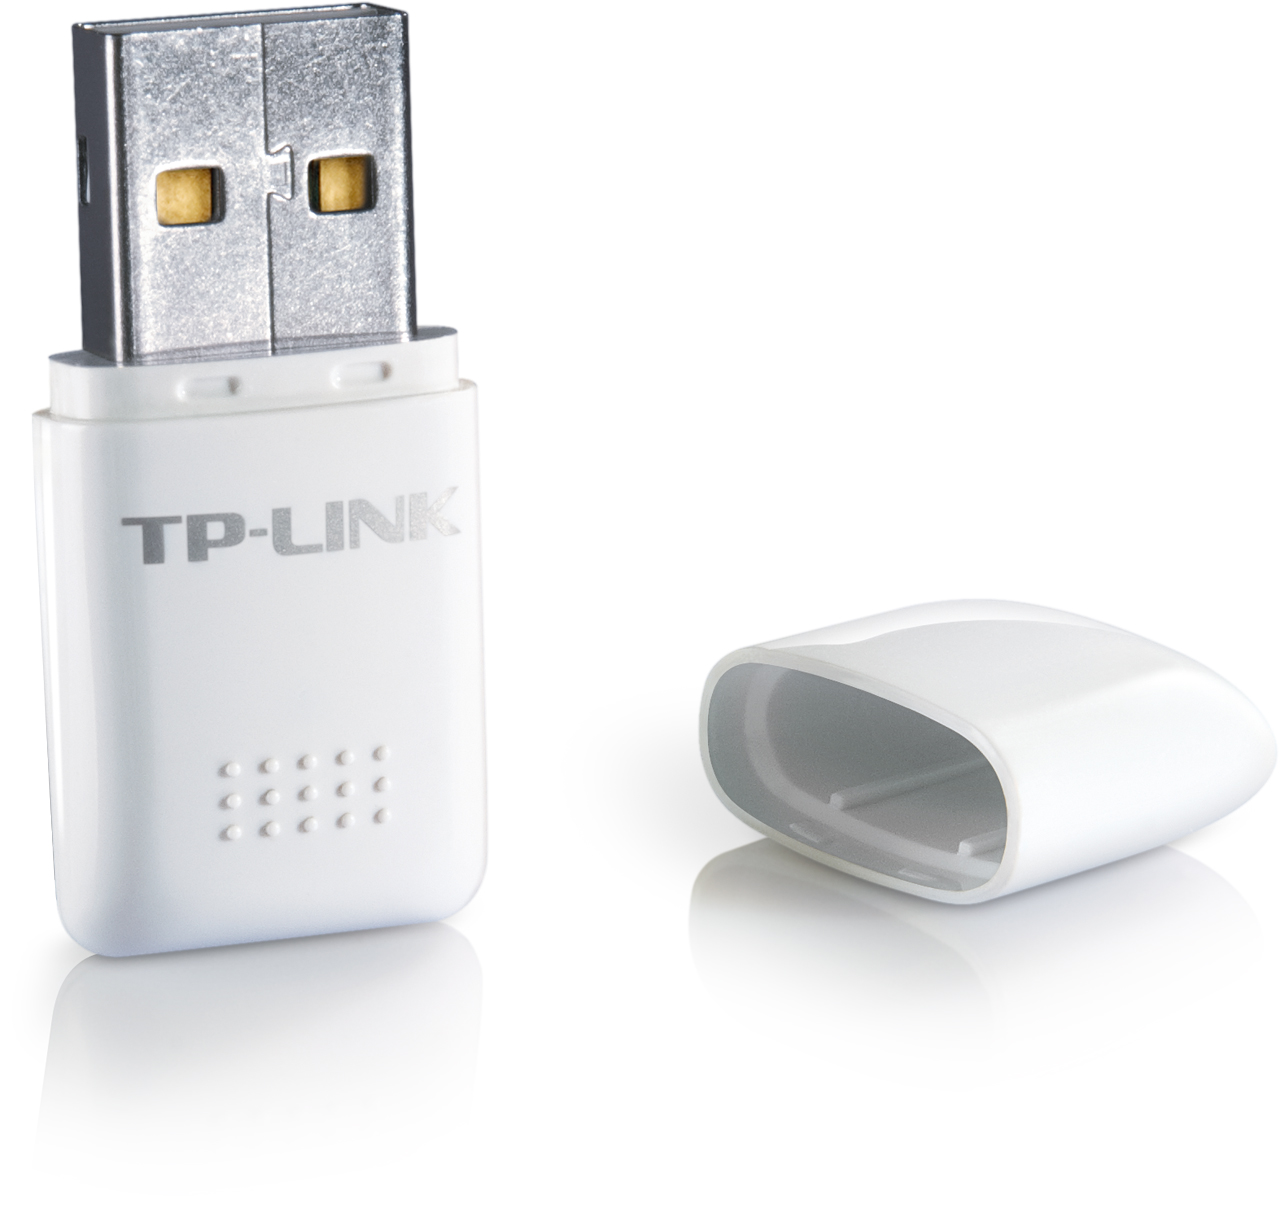
\includegraphics[width=5cm,height=5cm,keepaspectratio]{figuras/wifi-adapter.jpg}
\caption{\label{fig:wifi-adapter} Adaptador wifi usado no raspberry}
\end{figure}

\subsection{Raspberry x Arduino: comunicação}

Para testar a comunicação entre o Módulo Coordenador (figura \ref{fig:teste-inicial-raspberry}) e o módulo sensor (figura \ref{fig:teste-inicial-arduino}), foi montado o esquema representado na figura \ref{fig:teste-inicial-all} e foram executados dois programas. O programa \ref{lst:teste-inicial-arduino} foi utilizado no módulo sensor para transmitir o valor "123123" por um datagrama a ser enviado pela rede do XBee. Já o programa \ref{lst:teste-inicial-raspberry} foi utilizado no Módulo Coordenador para receber o datagrama ZigBee e imprimir no console do Raspberry.

\begin{figure}[H]
\centering
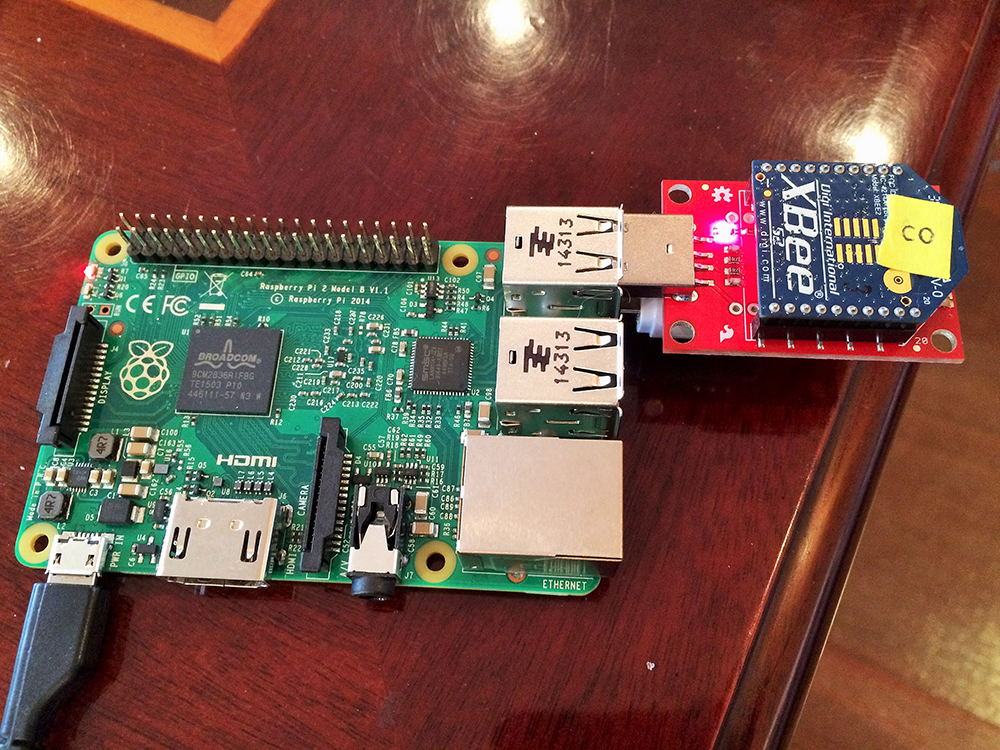
\includegraphics[width=7cm,keepaspectratio]{figuras/teste-inicial-raspberry.jpg}
\caption{\label{fig:teste-inicial-raspberry} Teste de comunicação: Módulo Coordenador}
\end{figure}

\begin{figure}[H]
\centering
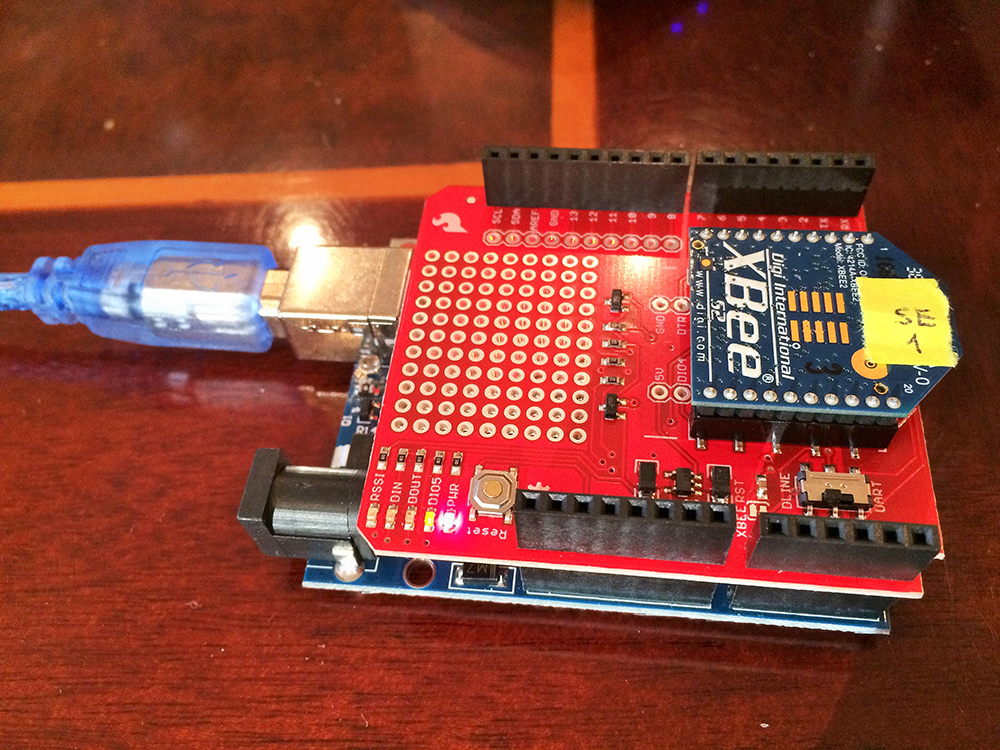
\includegraphics[width=7cm,keepaspectratio]{figuras/teste-inicial-arduino.jpg} 
\caption{\label{fig:teste-inicial-arduino} Teste de comunicação: Módulo Sensor}
\end{figure}

\begin{figure}[H]
\centering
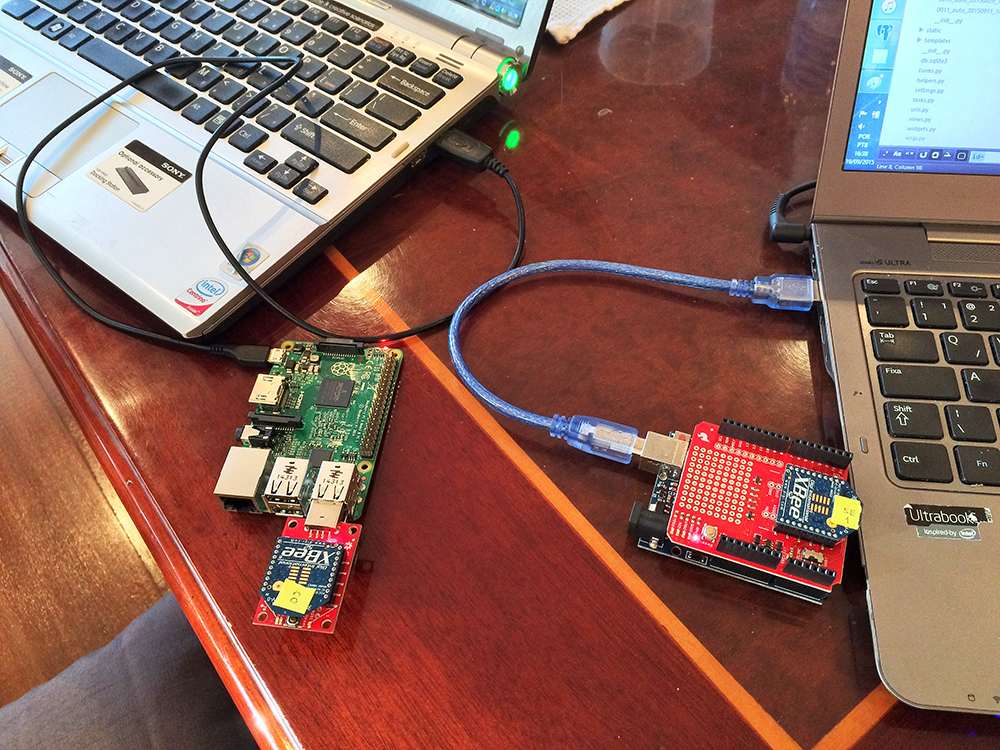
\includegraphics[width=7cm,keepaspectratio]{figuras/teste-inicial-all.jpg} 
\caption{\label{fig:teste-inicial-all} Teste de comunicação: Montagem}
\end{figure}

\lstinputlisting[language=C, caption=teste-inicial-arduino.c, label={lst:teste-inicial-arduino}]{Anexos/teste-inicial-arduino.c}

\lstinputlisting[language=Python, caption=teste-inicial-raspberry.py, label={lst:teste-inicial-raspberry}]{Anexos/teste-inicial-raspberry.py}

\begin{figure}[H]
\centering
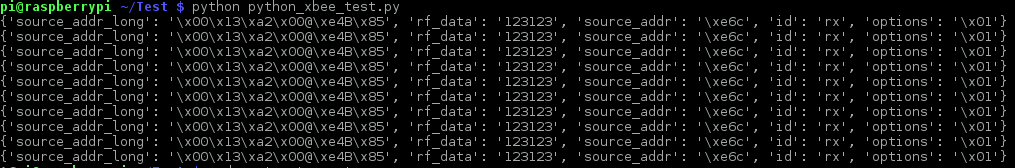
\includegraphics[width=1\textwidth]{figuras/teste-inicial-raspberry-arduino.png}
\caption{\label{fig:raspberry-arduino-1} Teste de comunicação Raspberry e Arduino}
\end{figure}

Após esse teste, foi feito um pequeno teste para observar o que ocorre com multiplos módulos sensores no sistema. Logo, o teste acima foi realizado com dois módulos com frequências diferentes de envio para garantir que não ocorre colisão.

\subsection{Verificador de tensão}

Para verificar a tensão foi usado um transformador para rebaixar a tensão da tomada. Na imagem é possível observar uma tomada de 127V sendo rebaixada para 7,2 V.

\begin{figure}[H]
\centering
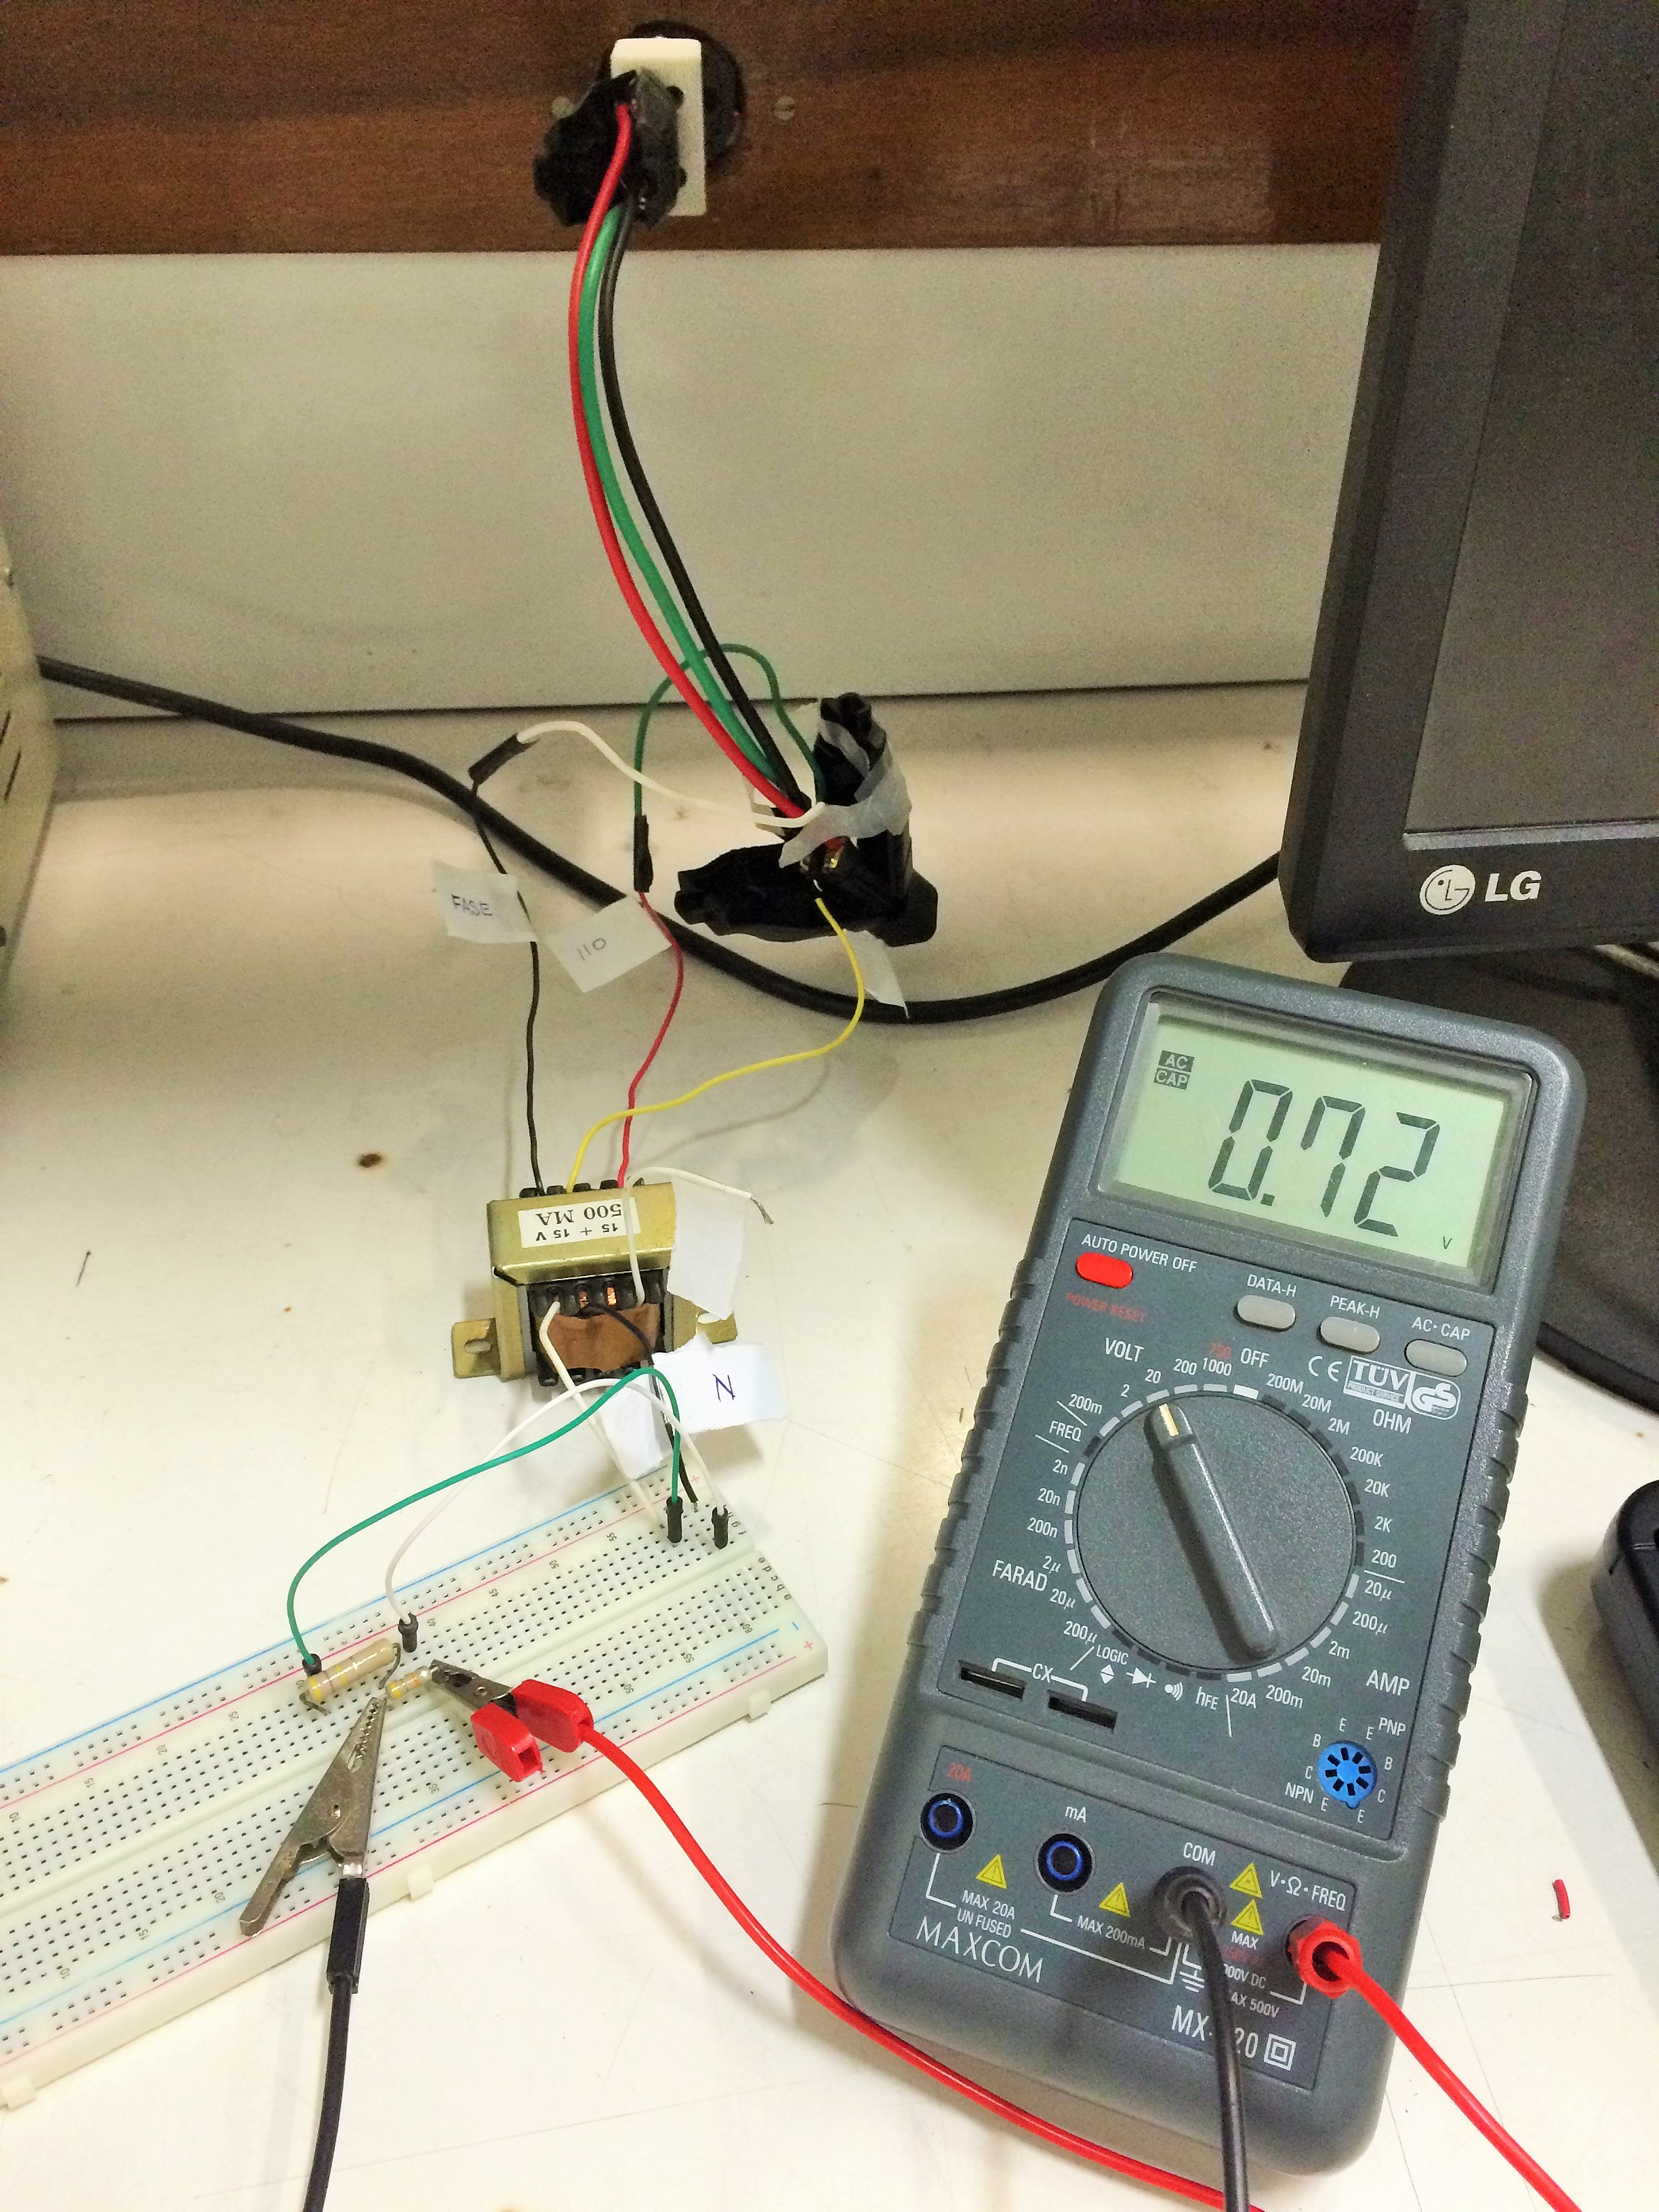
\includegraphics[width=7cm,keepaspectratio]{figuras/sensor-tensao.jpg} 
\caption{\label{fig:sensor-tensao} Teste do transformador}
\end{figure}

Em seguida a saída foi retificada com um retificador de onda completa e filtrada com um capacitor e dividida por divisão de tensão com resistores para que fosse possível diferenciar uma tensão de 220V e 127V no arduino para enviar ao raspberry.

A figura \ref{fig:teste-medicao-voltagem} mostra a montagem para tal e a figura \ref{fig:teste-medicao-voltagem-osc} mostra a saída no osciloscópio.

\begin{figure}[H]
\centering
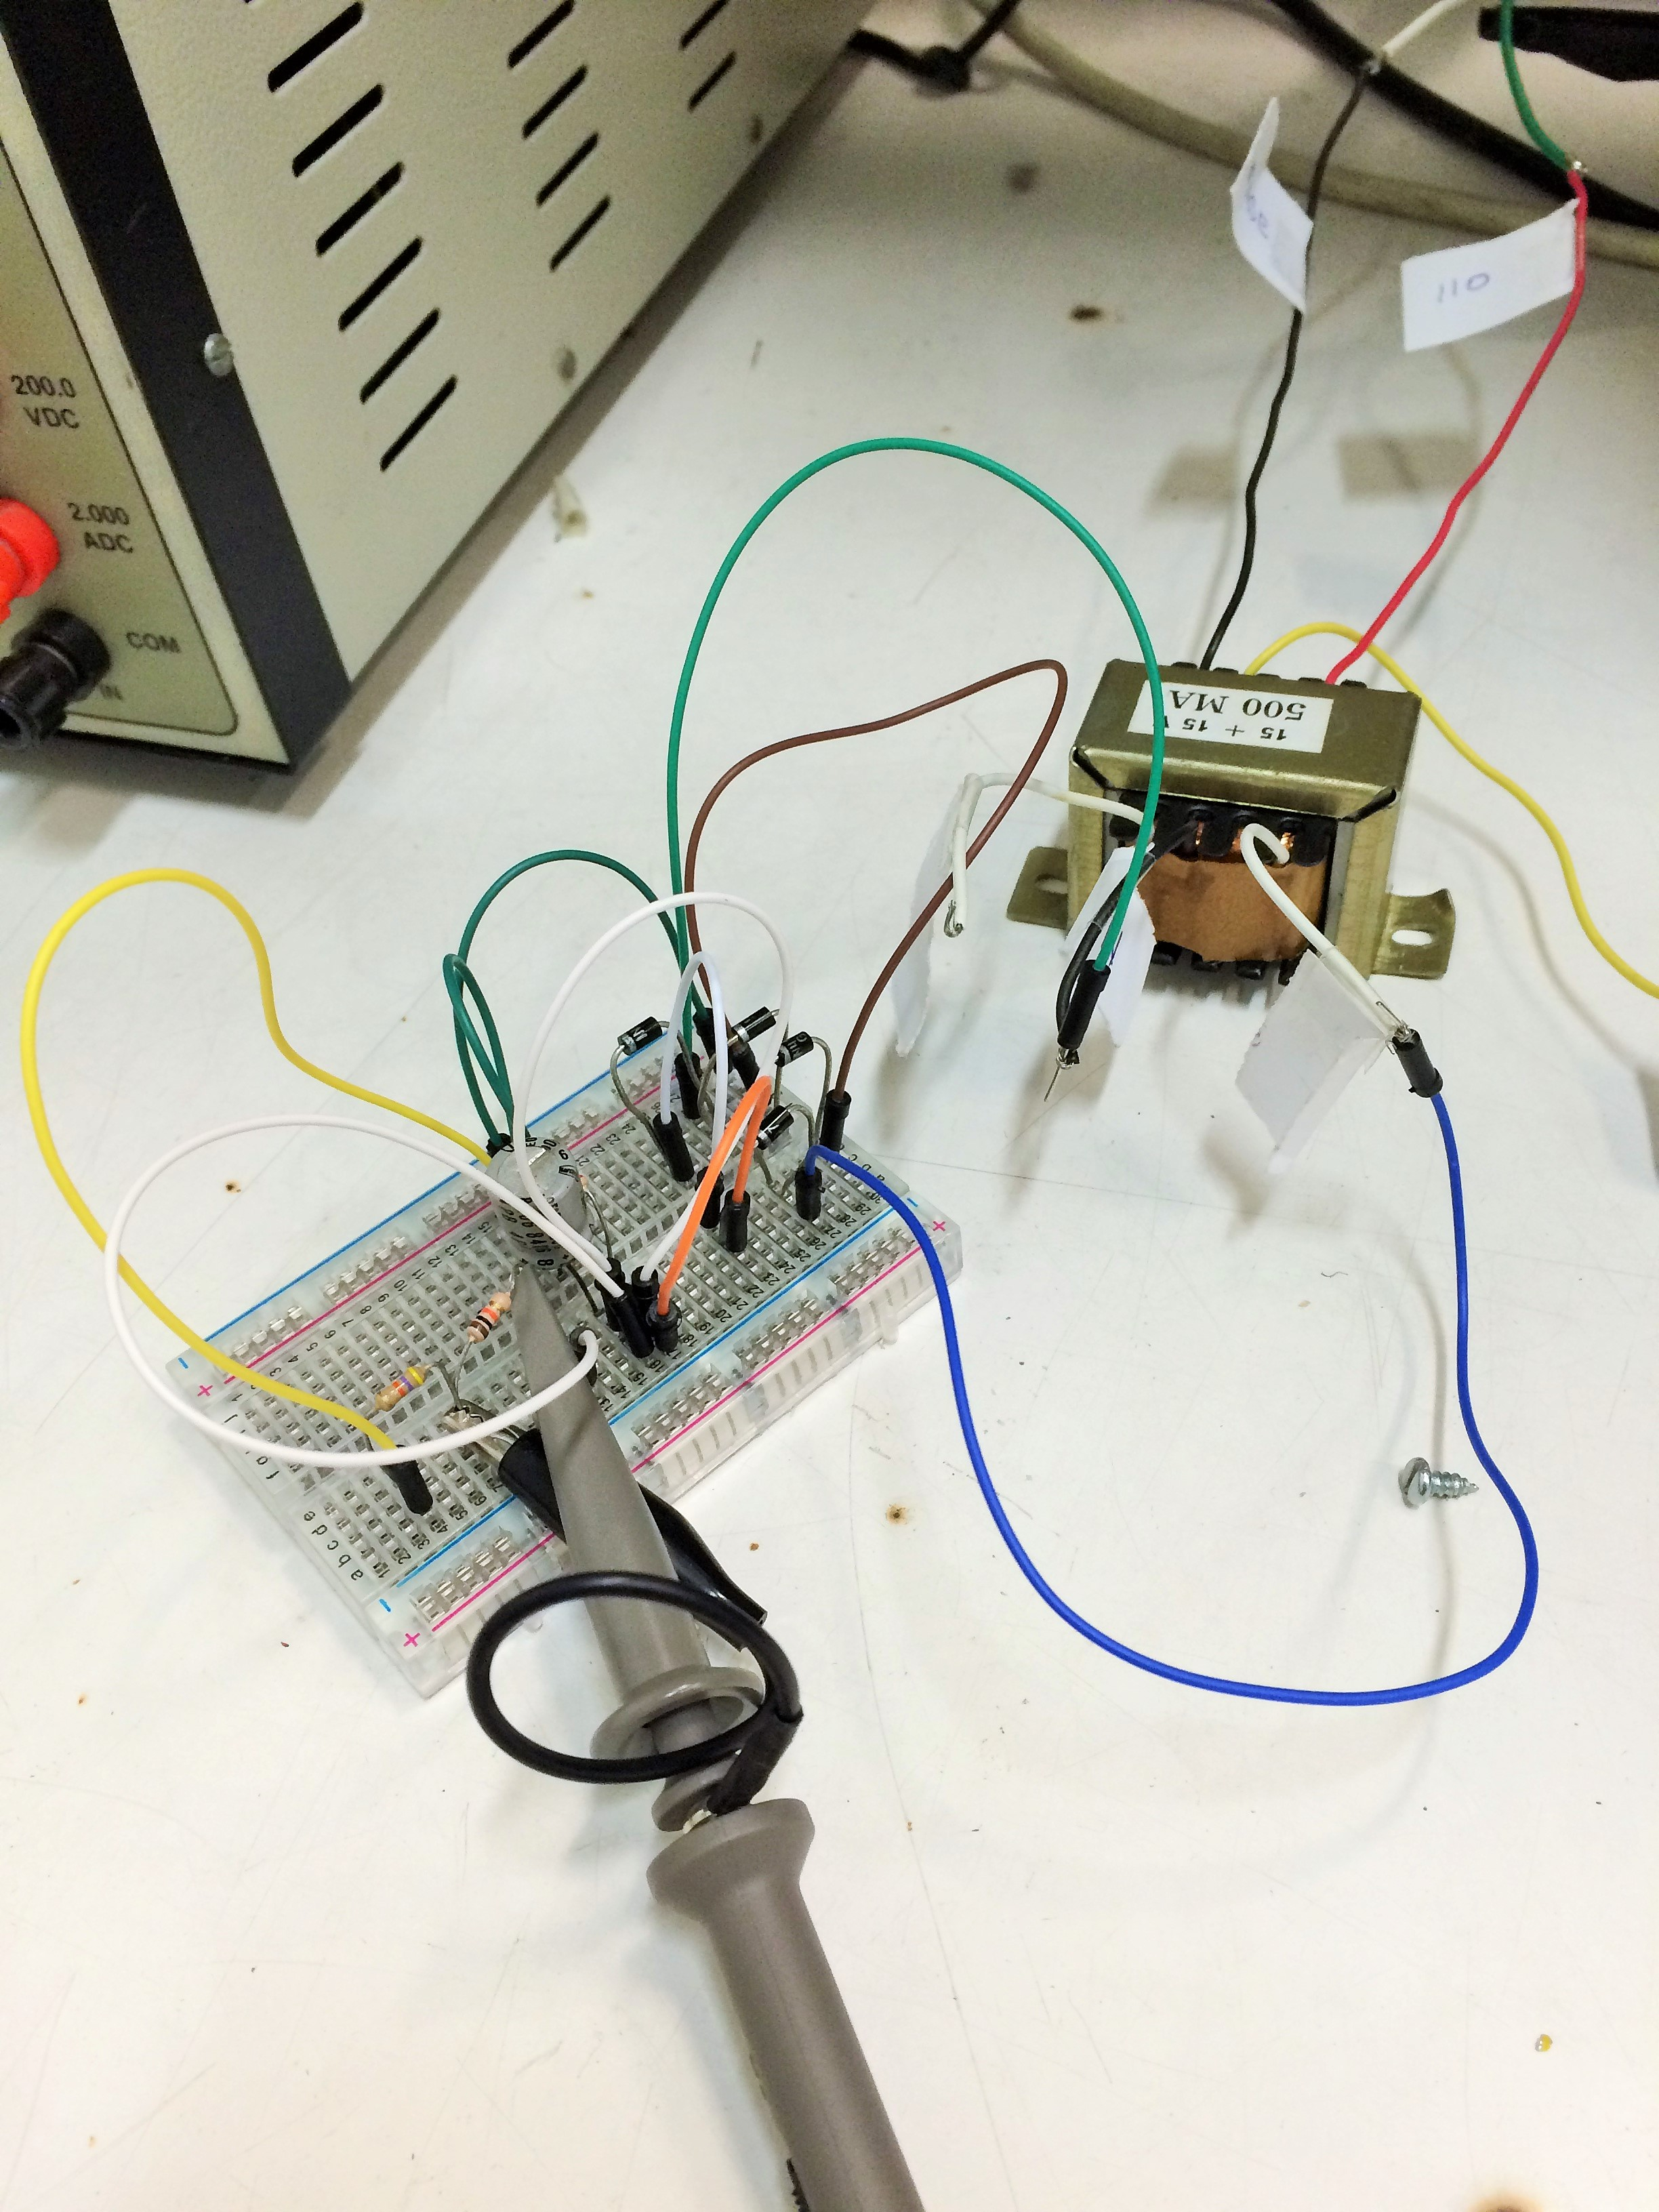
\includegraphics[width=7cm,keepaspectratio]{figuras/teste-medicao-voltagem.jpg} 
\caption{\label{fig:teste-medicao-voltagem} Teste de medição de tensão} 
\end{figure}

Em seguida a saída retificada e dividida foi posta como entrada para um pino de leitura analógica do Arduino para a medição, para 127V e em seguida, 220V. A saída resultante no terminal serial do arduino \ref{fig:teste-medicao-voltagem-osc} foi a seguinte

\begin{figure}[H]
\centering
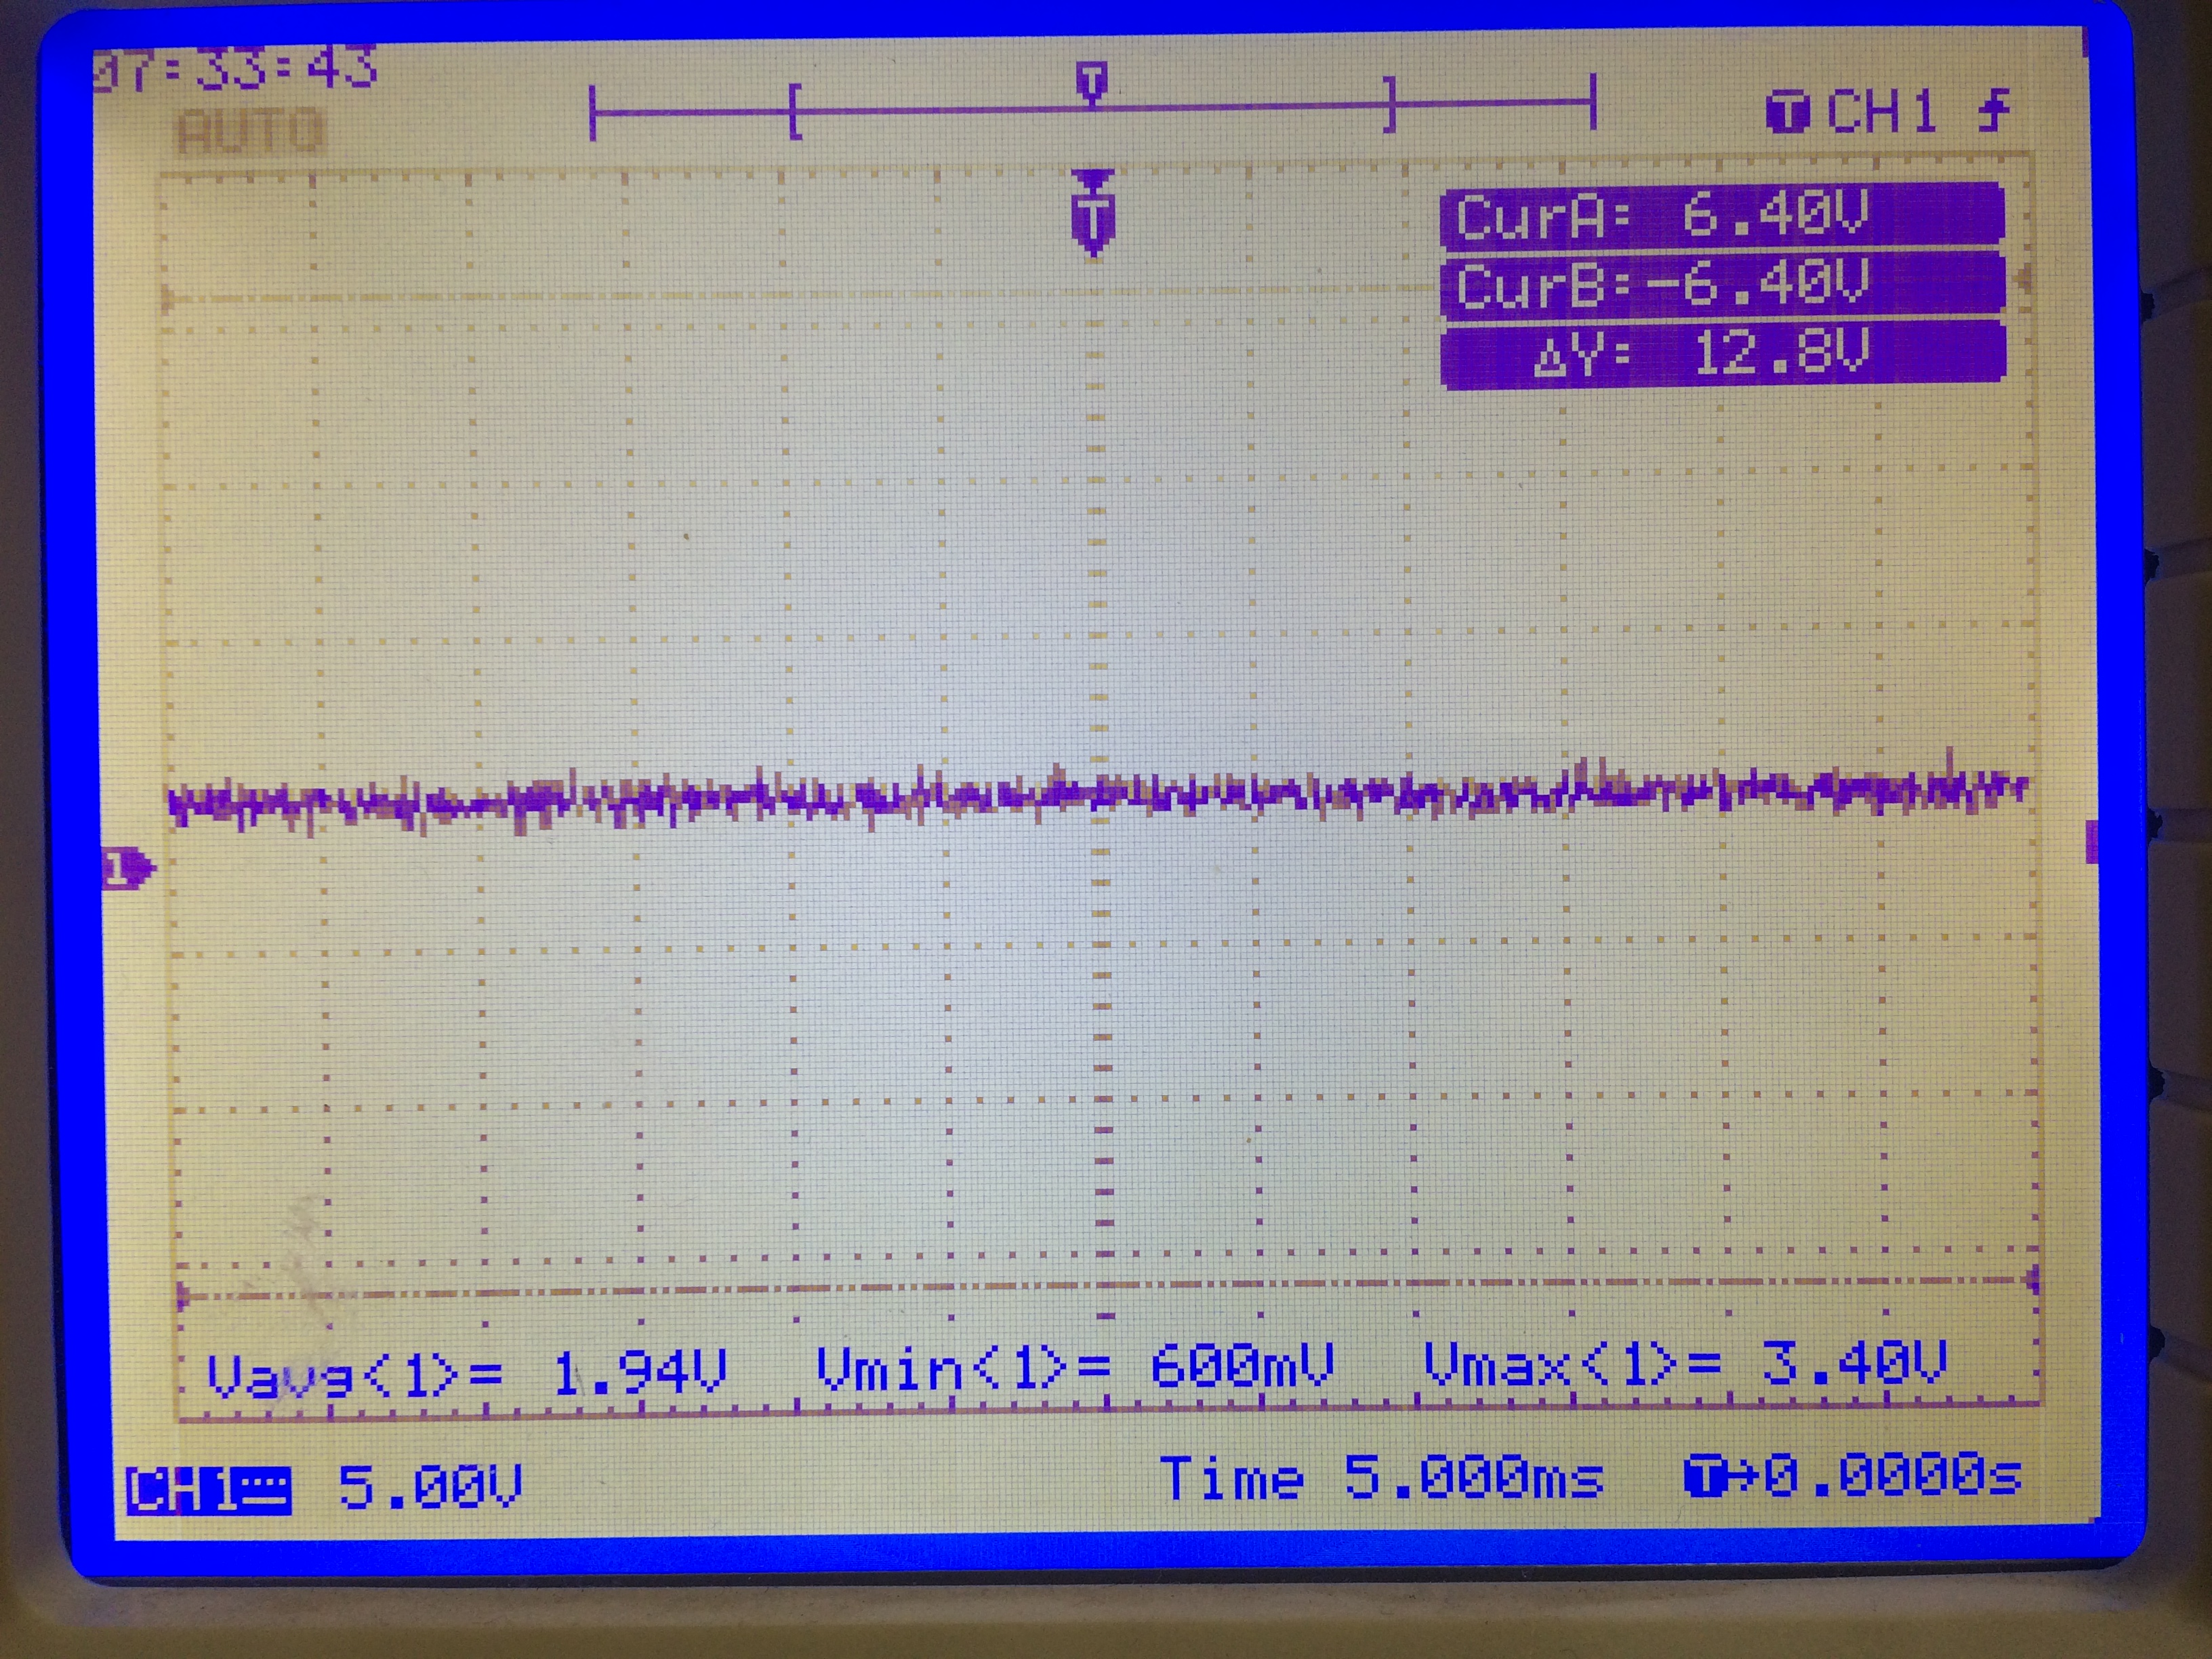
\includegraphics[width=7cm,keepaspectratio]{figuras/teste-medicao-voltagem-osc.jpg} 
\caption{\label{fig:teste-medicao-voltagem-osc} Teste de medição de tensão com arduino - saída do osciloscópio}
\end{figure}

\subsection{Sensor de corrente}

Para o sensor de corrente, dado que a saída do sensor é alternada, foi necessário fazer um pequeno circuito para que as informações coletadas estivessem em uma faixa legível ao arduíno. Para isso, foi colocado uma resistência entre as saídas do sensor, resistência essa que deveria, em 30A (corrente máxima do sensor), resultar em uma tensão máxima de 2,5V para então adicionar um offset de 2,5V, possibilitando amostragens em todos os pontos da onda. Como apenas o valor de pico é relevante para calcular a potência aparente.
No caso, a resistência utilizada foi de 150 omhs. 

Já no arduino, para fazer a leitura, não era possível apenas ler diretamente o valor da entrada analógica, pois estávamos interessados no valor eficaz da corrente. Por isso foi utilizado da raiz da média dos quadrados (tradução livre de RMS - root mean square), fazendo várias leituras sucessivas, assim como o nome do método diz, faz-se a raiz da média dos quadrados das leituras para obter o valor eficaz.

Com o circuito de corrente pronto, foi possível fazer algumas leituras teste. No caso foi usado o ferro de passar para que fosse usada uma corrente mais alta. 

Como se pode ver nos testes, apesar da corrente lida no amperímetro ser 9,3A eficazes (figura \ref{fig:teste-amperimetro}), as leituras no arduíno resultaram em valores ligeiramente menores entre 8,9 e 8,8A eficazes (figura \ref{fig:teste-medicao-corrente-voltagem}), resultando em um erro de aproximadamente 7\%, que é um erro relativamente alto se pensado em uma leitura de longo prazo.

\begin{figure}[H]
\centering
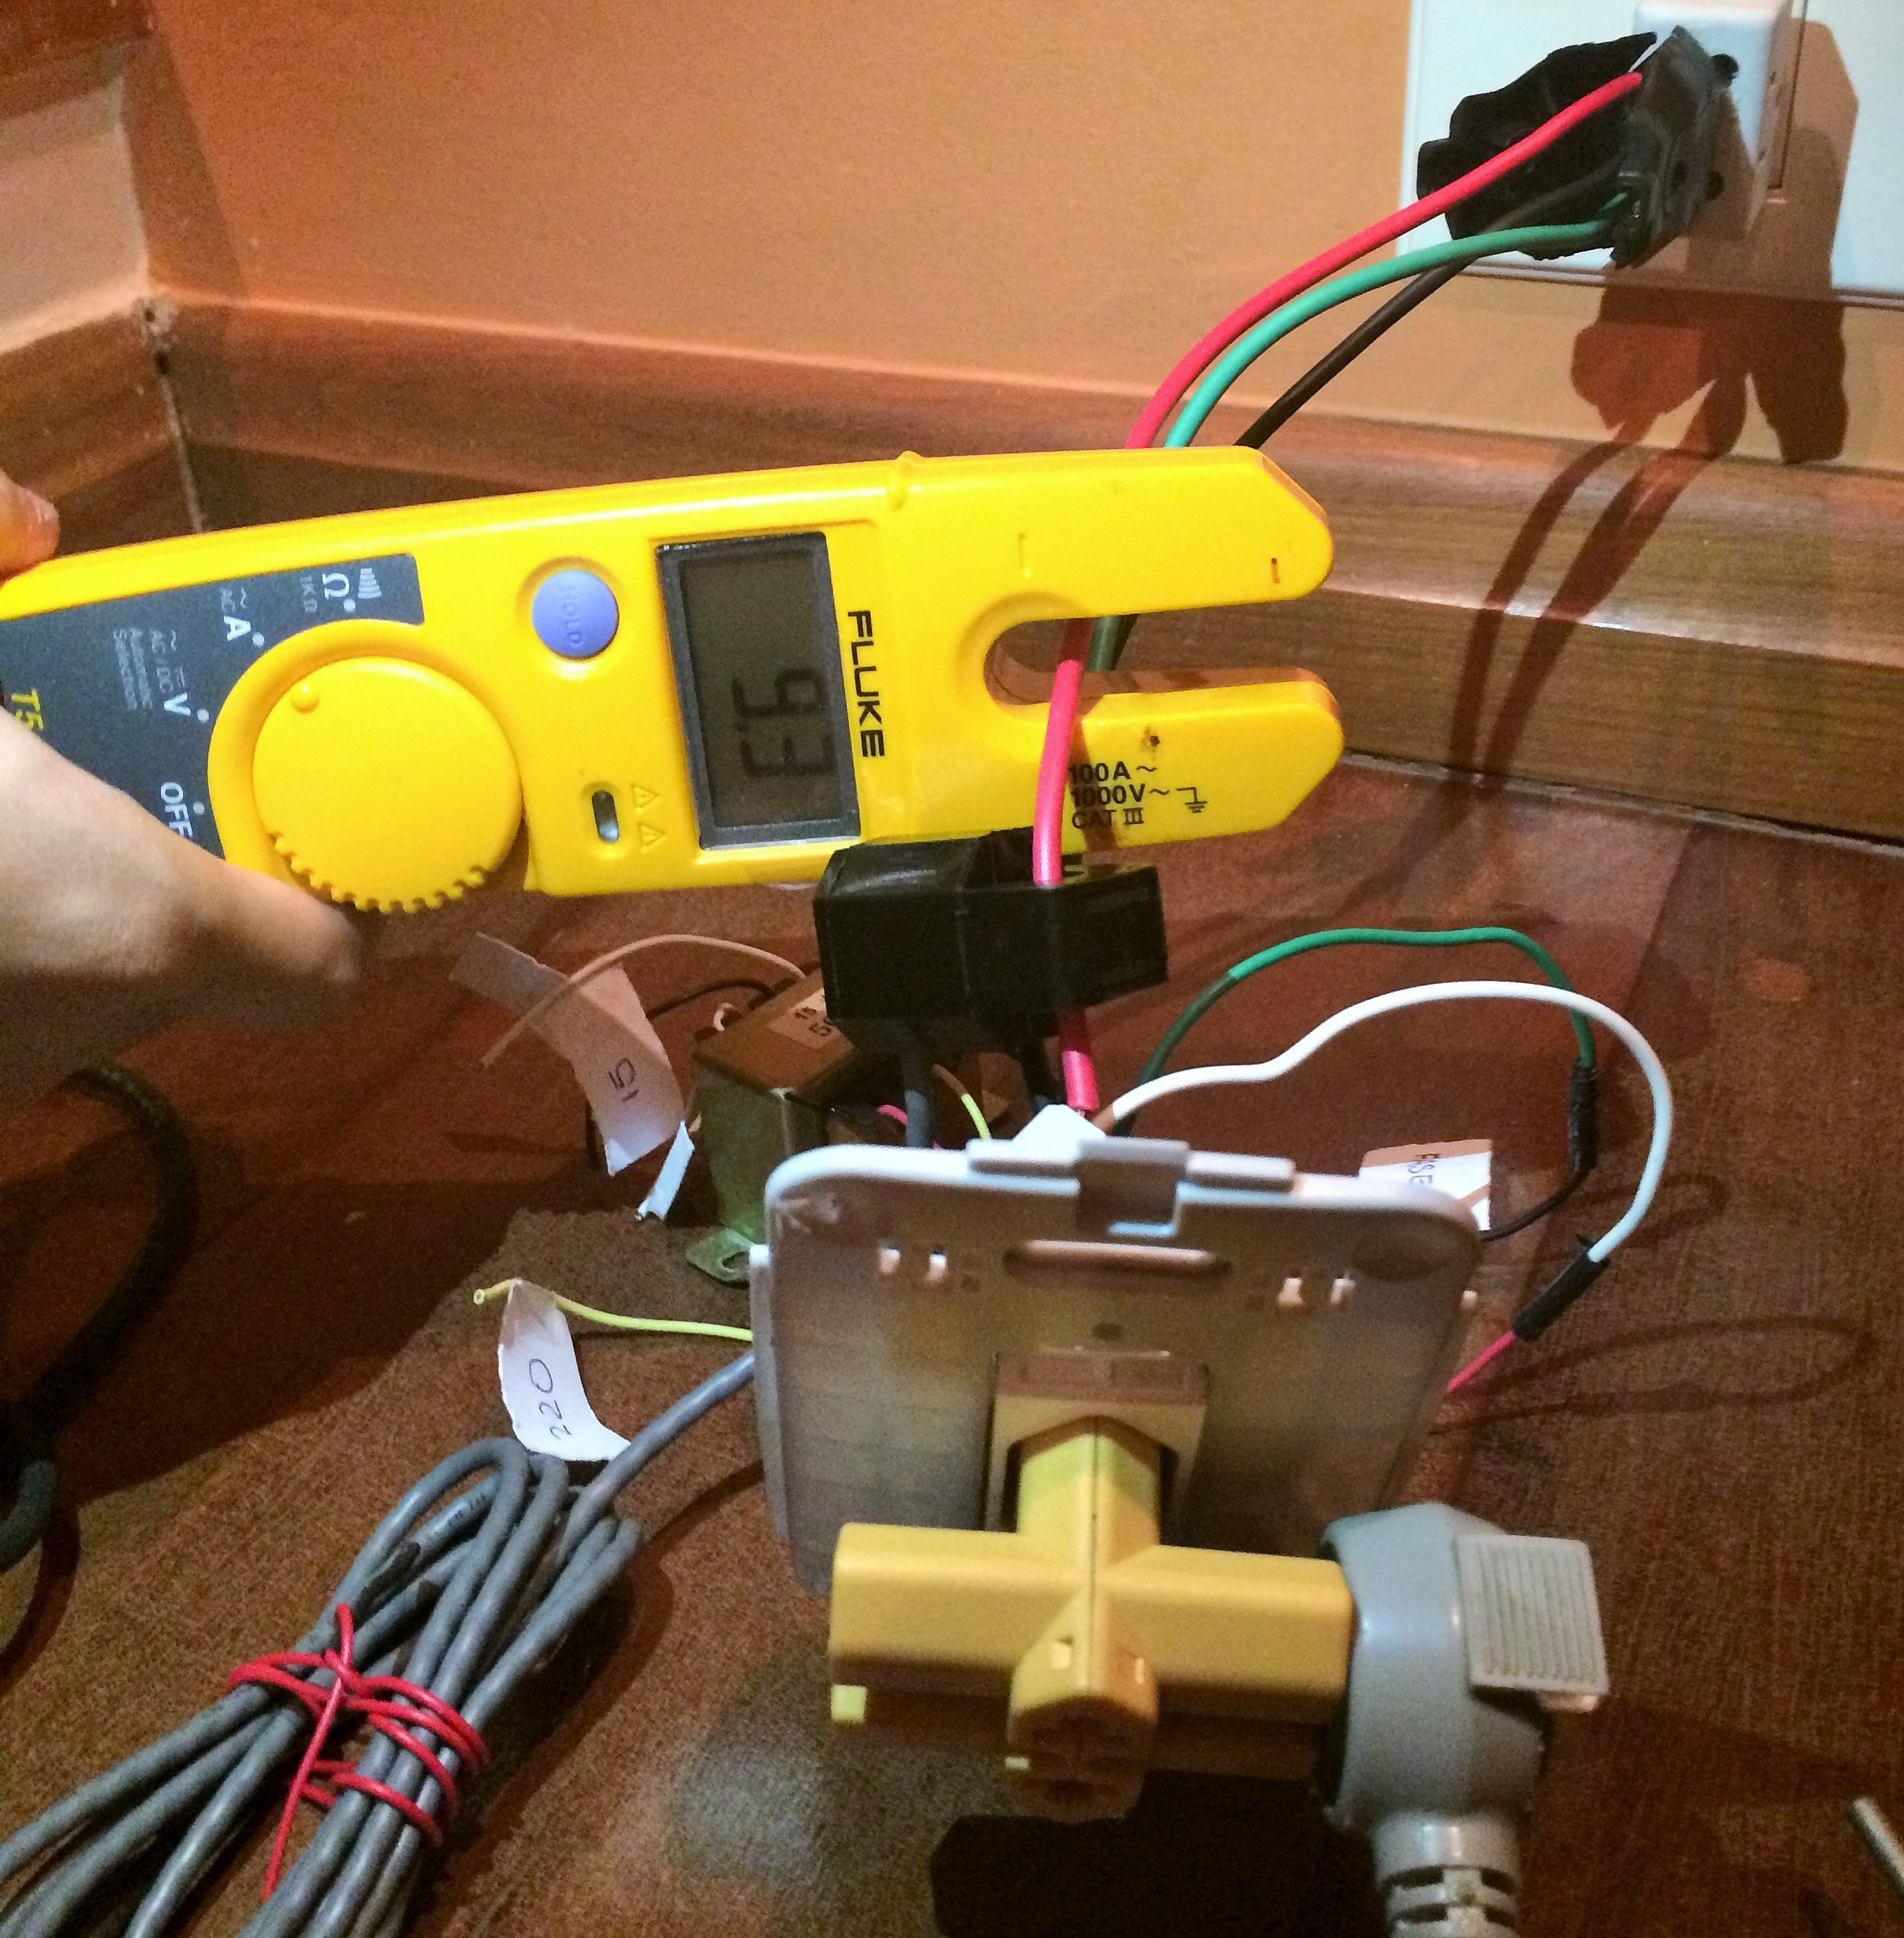
\includegraphics[width=7cm,keepaspectratio]{figuras/ferro-passar-amp.jpg} 
\caption{\label{fig:teste-amperimetro} Medição com amperímetro}
\end{figure}

\lstinputlisting[language=C++, caption=Leitura da corrente, label={lst:Leitura da corrente}]{Anexos/voltage_and_current.ino}

\begin{figure}[H]
\centering
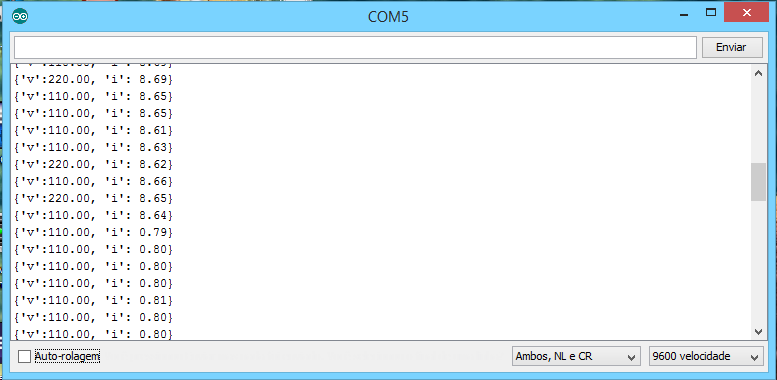
\includegraphics[width=10cm,keepaspectratio]{figuras/ferro-passar.png} 
\caption{\label{fig:teste-medicao-corrente-voltagem} Teste de medição da corrente e tensão}
\end{figure}

\subsection{Integrando as partes}

Após os testes anteriores de comunicação entre o módulo sensor, módulo coordenador e a medição de corrente e tensão, o conjunto foi testado. O código \ref{lst:arduino-code} foi carregado no arduino para a coleta dos dados de corrente e tensão e o envio destes para o módulo coordenador.

\lstinputlisting[language=C, caption=arduino.c, label={lst:arduino-code}]{Anexos/arduino.c}

O módulo coordenador foi configurado para executar o seguinte programa em python (código \ref{lst:raspberry-code}), logo após ligar o raspberry, para a inicialização da interface entre os sensores e a aplicação web. Uma vez com o programa em execução, o módulo coordenador estará pronto para escutar as requisições de envio de dados coletados dos módulos sensores. 

\lstinputlisting[language=Python, caption=raspberry.py, label={lst:raspberry-code}]{Anexos/raspberry.py}

A idéia dos códigos é que o arduino envie seu endereço MAC para diferenciá-lo na rede e uma string formatada como um JSON para que esse seja convertido no raspberry e as informações sejam extraídas.
